\chapter{RADAR}
 この章ではRADARの基本原理,研究に使用するRADARの性能を示し,LiDARとの比較を行う.

\section{RADARの概要}
 RADARは電波を発射し遠方にある目標物を検知し,そこまでの距離を測る電波検知装置である\cite{RADAR_book}.\\
 RADARシステムは以下のような簡易なブロック図(図\ref{fig:RADAR_Block})で表される.

\begin{itemize}
    \item \textbf{送信アンテナ部}\\
        電波を効率よく物標に放射し,反射波を捉える装置
    \item \textbf{信号処理部}\\
        受信したデータ列を検出や測距など目的を達するために行うソフトウェア処理
    \item \textbf{検波部}\\
        受信波を信号処理しやすい信号形式に変換する装置
\end{itemize}

\begin{figure}[H]
    \centering
    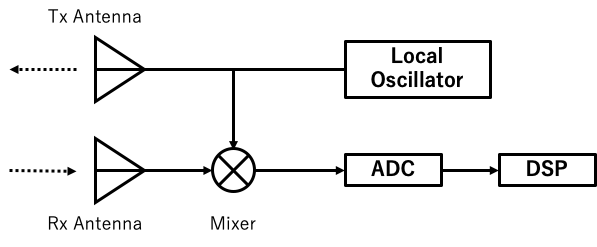
\includegraphics[width=8.5cm]{./fig/RADAR_Block.png}
    \caption{RADARのブロック図}
    \label{fig:RADAR_Block}
\end{figure}

 例えば,RADARではパルス波(矩形波)を図\ref{fig:RADAR_Demo}のように物標方向に照射し,その反射信号から距離に対する反射強度を得ることができる.物標の位置はこの反射波の強度のピークが発生している箇所に存在すると考えることができる.なお,この反射強度は物体の比誘電率に依存する.障害物のない箇所でも空気による若干の反射は発生するが,空気の比誘電率は物標より小さくなるため反射は少なくなり,物標の検知が可能となる.

\begin{figure}[H]
	\subfigure{%
		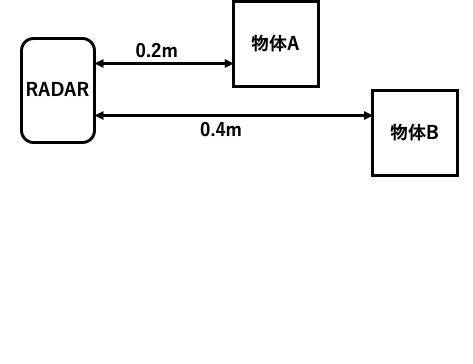
\includegraphics[clip, width=0.35\columnwidth]{./fig/RADAR_Demo.png}}%
	\subfigure{%
		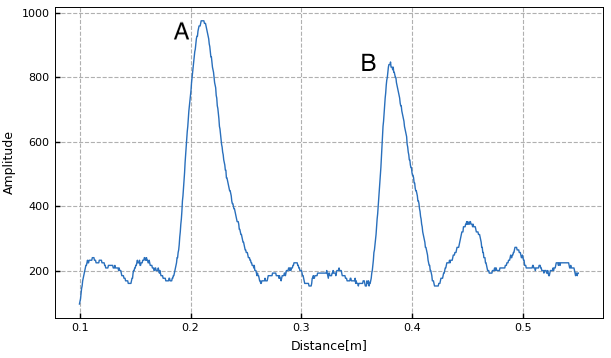
\includegraphics[clip, width=0.65\columnwidth]{./fig/RADAR_Demo_Graph.png}}%
	\caption{物体の位置と反射強度の関係}
	\label{fig:RADAR_Demo}
\end{figure}


\section{ミリ波}
 ミリ波の波長は図\ref{fig:ClassificationOfRadioWaves}に示すように1mm~10mmと非常に短い.
\begin{figure}[H]
    \centering
    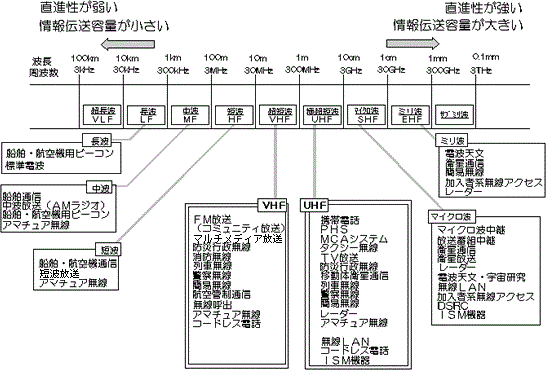
\includegraphics[width=10cm]{./fig/ClassificationOfRadioWaves.png}
    \caption{電波の分類\cite{soumu_RadioWaves}}
    \label{fig:ClassificationOfRadioWaves}
\end{figure}

 波長が1cm以下のマイクロ波と比較した際の特徴を以下に述べる\cite{feature_RadioWaves}.
\begin{enumerate}
    \item \textbf{広帯域性}\\
        RADARの分解能は帯域幅の逆数となる.ミリ波は広い帯域幅を利用できるため高分解能・高精度化が可能となる.
    \item \textbf{装置の小型軽量化}\\
        アンテナ開口径は波長に比例するため,周波数が高いほど装置サイズを小さくできる.
    \item \textbf{鋭い指向性}\\
        空間的に高密度の利用が可能となる.また,お互いの電波の干渉も低くできる.
\end{enumerate}

\section{本研究で使用するRADAR}
 本研究ではAcconeer社製のXC112/XR112評価キットを用いる.この評価キットは同社製のA111というパルスRADARを搭載したRADARセンサボード(XR112)とRaspberryPiとの接続用コネクタボード(XC112)から構成される.図\ref{fig:XC112},図\ref{fig:XR112}にXC112およびXR112の外観を示す.
\begin{figure}[H]
    \centering
    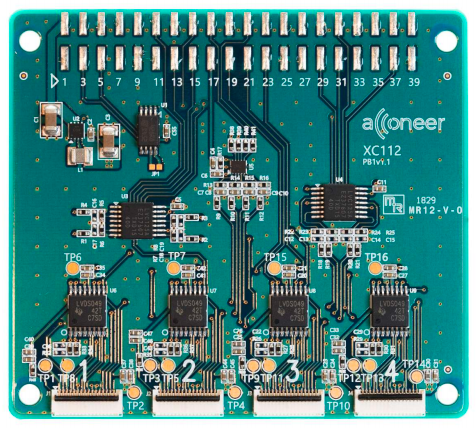
\includegraphics[width=6cm]{./fig/XC112.png}
    \caption{XC112\cite{XC112ProductBrief}}
    \label{fig:XC112}
\end{figure}

\begin{figure}[H]
    \centering
    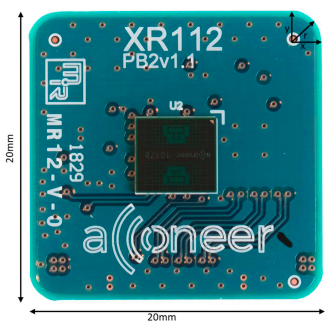
\includegraphics[width=4cm]{./fig/XR112.png}
    \caption{XR112\cite{XR112ProductBrief}}
    \label{fig:XR112}
\end{figure}

評価キットのブロック図を図\ref{fig:EVK_Block}に示す.
\begin{figure}[H]
    \centering
    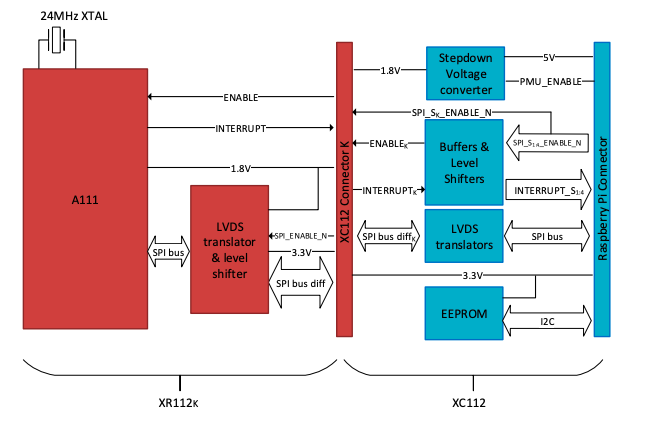
\includegraphics[width=8.5cm]{./fig/EVK_Block.png}
    \caption{XC112/XR112評価キットのブロック図\cite{XC112_XR112UserGuide}}
    \label{fig:EVK_Block}
\end{figure}

 シングルボードコンピュータのRaspberryPiを使用することを想定しており,本研究でもRaspberryPi3 ModelBをRADAR制御用コンピュータとして使用した.評価キットに使用されているA111は周波数60GHz(波長 5 mm)のミリ波RADARである\cite{XC112_XR112UserGuide}.
